\documentclass[a4paper,12pt]{amsart}
\usepackage[T1, T2A]{fontenc}

\usepackage[utf8]{inputenc}

\usepackage{amsmath}
\usepackage{amsthm}
\usepackage{relsize}
\usepackage{graphicx}
\usepackage{amssymb,stackengine}

%\usepackage[english]{babel}
\usepackage[ukrainian, english]{babel}

\usepackage{listings}
% \usepackage[colorlinks]{hyperref}
\usepackage{hyperref}
\usepackage[title]{appendix}


% template
\frenchspacing \righthyphenmin=2 \emergencystretch=5pt
\hfuzz=0.5pt \tolerance=400 \oddsidemargin 5mm \evensidemargin 5mm
\textwidth 160mm \textheight 230mm

\hoffset=-0.5cm \voffset=-1.0cm

%\renewcommand\baselinestretch{1.1}



\usepackage{xcolor}

% links
\hypersetup{
	colorlinks=true,
	linkcolor=blue,
	filecolor=magenta,
	urlcolor=cyan,
}

% coloring of listings


\definecolor{codegreen}{rgb}{0,0.7,0}
\definecolor{codegray}{rgb}{0.4,0.4,0.4}
\definecolor{codepurple}{rgb}{0.58,0,0.82}
\definecolor{backcolour}{rgb}{0.95,0.95,0.92}

\lstdefinestyle{mystyle}{
	backgroundcolor=\color{backcolour},
	commentstyle=\color{codegray}\textit,
	keywordstyle=\color{magenta},
	numberstyle=\tiny\color{codegray},
	stringstyle=\color{codepurple},
	%	basicstyle=\ttfamily\footnotesize,
	breakatwhitespace=false,
	breaklines=true,
	captionpos=b,
	keepspaces=true,
	numbers=left,
	numbersep=3pt,
	showspaces=false,
	showstringspaces=false,
	showtabs=false,
	tabsize=2
}

\lstset{style=mystyle}


% path to images
\graphicspath{ {../../graphs/} }

\usepackage[left=2.5cm,right=3cm,
    top=2cm,bottom=2cm,bindingoffset=0cm]{geometry}
    
\title{ 	Складність проблеми слів в Ханойських групах }
\author{ David Zashkolny }
\date{March 2020}

\newtheorem{definition}{Definition}
\newtheorem{corollary}{Corollary}
\newtheorem{hypothesis}{Conjecture}
\newtheorem{proposition}{Proposition}

\newtheorem{theorem}{Theorem}
\newtheorem{lemma}{Lemma}


\begin{document}


\thispagestyle {empty}
\begin{center}
	\large  Київський Національний Університет імені Тараса Шевченка \\
	Механіко-математичний факультет \\
	Кафедра алгебри і комп'ютерної математики \par
\end{center}


\begin{center}
	\vskip0cm plus 2fill
	\vspace{2.5cm} {\bf Курсовий проект}\\

	%{\bf на здобуття ступеня магістра математики}\\
	{\bf на тему:}\\
\end{center}


\vskip0cm plus 1.0fill



\begin{center}\bf
	{\LARGE
		The word and order problems in Hanoi Tower Groups \par}
\end{center}

\vskip0cm plus 1.5fill

\hangindent=7cm \hangafter=0 \noindent
Виконав\\
студент 4-го курсу\\
напрям математика\\
спеціалізація "комп'ютерна математика"\\
{\bf Зашкольний Давид Олександрович}\\[2cm]
Науковий Керівник:\\
Доцент кафедри, доктор фiзико-математичних наук\\
{\bf Бондаренко Євген Володимирович}


\vskip0cm plus 1.5fill

\vskip5cm plus 1.5fill
\begin{center}
	КИЇВ --- 2021
\end{center}

\newpage
\pagenumbering{arabic}

%\newpage
\tableofcontents

\newpage

\section{Introduction}
This article is focused on combinatorial properties of some automaton groups, particularly of so-called Hanoi Tower Groups $H_k$ that appear in various mathematical fields and could be defined in couple different ways. The majority of considered properties connected with \textbf{the word problem} that is one of three classical decision problems for finitely generated groups. There were proposed algorithms for solving the word and order problems in $H_k$, the correctness of working was proven and complexity in the worst case in $H_3$ was found.

Another goal of this work was to develop a decent Python framework for working with automaton groups at all and particularly with Hanoi Tower ones. More specifically, there were implemented classes for convenient work with elements of considered groups and set of tools to visualize some their properties, e.g. tree-like structure, process of algorithm solving the order problem etc. Should you want to see full implementation or try it for yourself, check \url{https://github.com/davendiy/automata-groups}.

\newpage

\section{General overview}

\subsection{Hanoi Tower Game and Automaton Groups} 

The Tower of Hanoi is a famous mathematical game that was invented by the French mathematician Édouard Lucas in 1883. A classical variant of the game is played with $n$ disks placed on three pegs. The objective of this game is to move all discs from one peg to another obeying one simple rule - a bigger disk can't be placed upon smaller one. It is a well-known fact that the minimal number of moves required to solve the game is $2^n - 1$. 


\begin{figure}[h]
	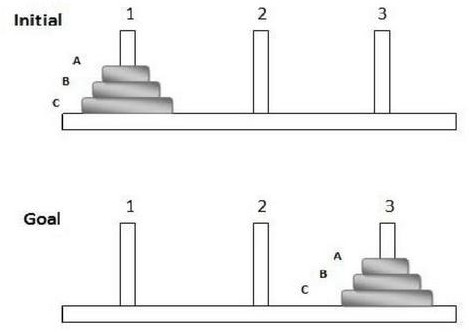
\includegraphics[scale=0.4]{hanoi_tower.jpg}
\end{figure}


A general version of the game is played with $n$ disks on $k$ pegs and in this case the minimal number isn't as obvious as in the previous one. Although the three-peg version has a simple recursive algorithm long been known, the optimal solution for the Tower of Hanoi problem with even four pegs was not verified until 2014, by Bousch \cite{Bousch}. Besides, a Frame-Stewart algorithm has been known without proof of optimality since 1941. \cite{Frame-Stewart}

Hereby fix alphabet $\Sigma_k = \{0, 1, \dots k\}$. Each word $w = x_1x_2\dots x_n \in \Sigma_k^n$ represents correct configuration of the game with $n$ disks on $k$ pegs assuming $x_i \in \Sigma_k$ means the number of peg whereon the $i$-th smallest disk is placed. 

Consider recursive functions $a_{(ij)} : \Sigma_k^* \rightarrow \Sigma_k^*$ as following (here $x \in \Sigma_k$ represents the first symbol): 

$$
a_{(ij)}(xw) = 
	\begin{cases}
	iw, \quad x = j \\
	jw, \quad x = i \\
	xa_{(ij)}(w), \quad x \notin \{i, j\}
	\end{cases}
$$	

It's easy to check that aforementioned functions can be naturally interpreted as allowable single disk move from one peg to another. Since all of them are bijections they generate a so-called \textit{Hanoi Tower Group} on $k$ pegs $H_{k}$ with identical function $e : \Sigma_k^* \rightarrow \Sigma_k^*$ as group's identity element and superposition as an action. \cite{Hanoi1}  

The group $H_k, \, k \ge 3$ is also an example of an automaton group. In general, an \textit{invertible automaton} is a quadruple $A = (S, X, \tau, \pi)$ where $S$ is a finite set of states, $X$ is a finite alphabet, $\tau: S\times X \rightarrow S$ a \textit{transition function} and $\pi : S \times X \rightarrow X$ an \textit{output function} such that, for each state $s \in S$, the restriction $\pi_s = \pi(s) : X \rightarrow X$ is a permutation in $S_X$ (see \cite{Auto}).  If, for instance, the automaton is complete and invertible then its states generate a group. 

Due to recursiveness of afore-defined functions elements of $H_k$ also have tree-like structure, i.e. $\forall w \in H_k \, w$ can be represented as follows: 

\begin{equation}
	\label{treelike}
	w = \pi (w_1, w_2, \dots w_k), \quad \pi \in Sym(\Sigma_k), w_i \in H_k
\end{equation}


\begin{figure}[h]
	\centering
	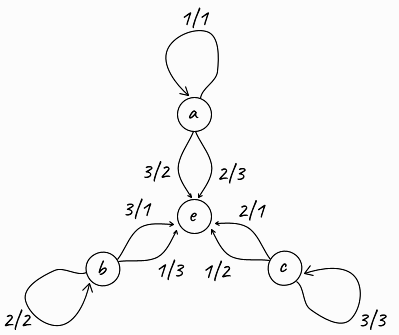
\includegraphics[scale=0.4]{H3_automaton.png}
	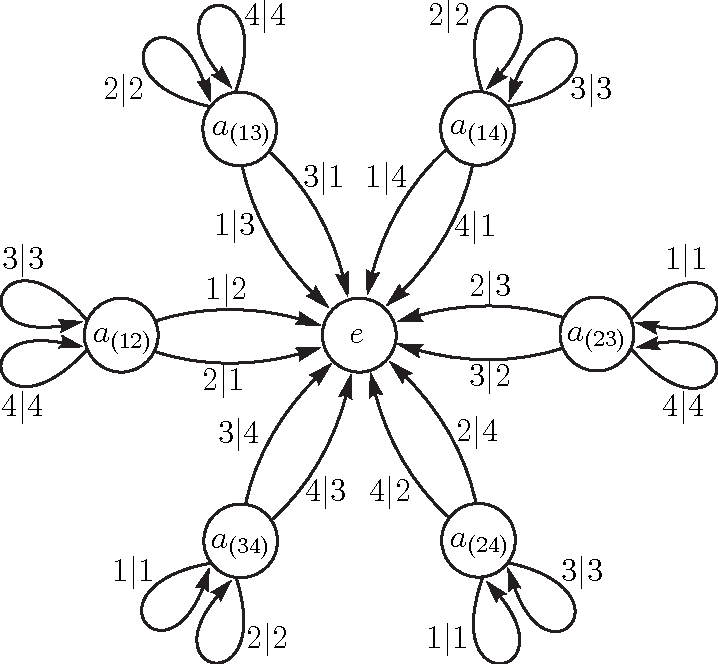
\includegraphics[scale=0.2]{H4_automaton.png}
	\caption{Automata for $H_3$ and $H_4$ respectively}
\end{figure}


Therefore, elements of the group denote a $k$-ary tree automorphisms whereby Hanoi Tower Group was originally defined in \cite{Hanoi1}. In \eqref{treelike} $\pi$ is called the \textit{root permutation} of $w$ while $w_i$ are called the (first level) \textit{sections} of $w$. 

Also, the multiplication rule is quite simple. Consider $g = \pi (g_1, g_2,\dots g_k), \, h = \sigma (h_1, h_2, \dots h_k)$ 

$$g*h = \pi * \sigma (g_{\sigma(1)}, g_{\sigma(2)}, \dots g_{\sigma(k)})$$

where permutations multiplies in a way $(\pi * \sigma)(x) = \sigma(\pi(x))$.
Hereafter, for simplicity, mark generators of $H_3$ as: 

$$ a := a_{(12)} = (1 2) (e, e, a_{(12)}) $$
$$ b := a_{(13)} = (1 3) (e, a_{(13)}, e) $$
$$ c := a_{(23)} = (2 3) (a_{(23)}, e, e) $$

and generators of $H_4$: 

% $$ a := a_{(23)} = (2 3) (a_{(23)}, e, e, a_{(23)}) $$
% $$ b := a_{(13)} = (1 3) (e, a_{(13)}, e, a_{(13)}) $$
% $$ c := a_{(12)} = (1 2) (e, e, a_{(12)}, a_{(12)}) $$
% $$ d := a_{(34)} = (3 4) (a_{(34)}, a_{(34)}, e, e) $$
% $$ f := a_{(24)} = (2 4) (a_{(24)}, e, a_{(24)}, e) $$
% $$ g := a_{(14)} = (1 4) (e, a_{(14)}, a_{(14)}, e) $$


$$ a := a_{(23)}, \, b := a_{(13)}, \, c := a_{(12)} $$
$$ d := a_{(34)}, \, f := a_{(24)}, \, g := a_{(14)} $$


Due to multiplication rule and defined generators it's obvious that $H_k$ is so-called \textit{contracting} group, i.e. $\forall w \in H_k, \, w = \pi (w_1, w_2, \dots, w_k) :\, |w_i| \le |w|$ and thus, each element of $H_k$ can be represented as finite k-ary tree. Hence, denote for every word $w$ over generators its tree as $T_w$.
Also define an operation called \textit{slice} of the word $w$ over generators recursively for any word over $\Sigma_k$ (possibly infinite): 

$$w|_x = w|_{x_0x_1\dots} = w_{x_0}|_{x_1\dots}, \quad x \in \Sigma_k^*, \, x_i \in \Sigma_k$$

\begin{figure}[h]
	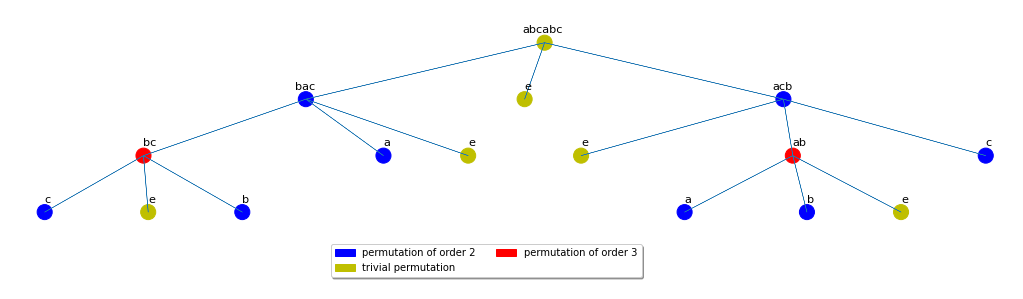
\includegraphics[scale=0.43]{abcabc.png}
	\caption{An example of tree-like structure in $H_3$}
\end{figure}

\begin{figure}[h]
	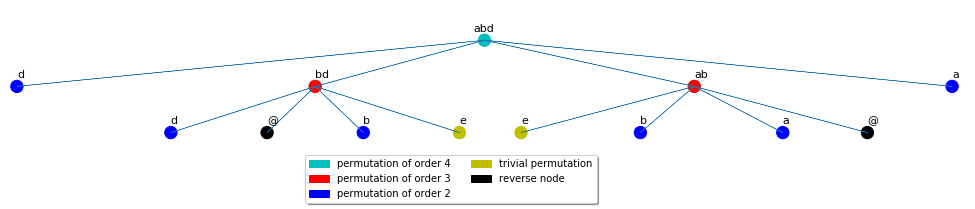
\includegraphics[scale=0.5]{abd.png}
	\caption{An example of tree-like structure in $H_4$}
\end{figure}

\subsection{Schreier Graphs}

Let finite generated group $G = \left\langle S \right\rangle$ act on a set $X$ where $S = \{g_1, g_2, \dots g_n\}$ - generators. Consider oriented graph $\Gamma(G, X, S) = (V, E)$ where $V = X$ is a set of vertices and $E = \{(x, g(x)) | \, x \in X, g \in S\}$ is a set of edges. $\Gamma(G, X, S)$ is called \textit{Schreier graph} of the group $G$ generated by $S$ acting on $X$. 

This graph is not always simple and connected though. Particularly in case of $H_k$ acting on $\Sigma_k^*$ the correspondent Schreier graph $\Gamma(H_k, \Sigma_k^*, \{a_{(ij)}, \, 1 \le i, j \le k\})$ has loops and can be divided on infinite amount of connected components $\Gamma_n(H_k, \Sigma_k^n, \{a_{(ij)}, \, 1 \le i, j \le k\})$ (hereby denote them as $H_k^n$) that represent action of $H_k$ on words over the alphabet $\Sigma_k$ of length $n$. Therefore, it's quite natural to consider the sequence of connected graphs $H_k^n$ instead of big one $\Gamma(H_k, \Sigma_k^*, \{a_{(ij)}, \, 1 \le i, j \le k\})$.

The sequence $H_3^n$ is simple and therefore it's been well-studied (\cite{Hanoi Graphs Random walks}, \cite{Hanoi2}). Here are some famous facts: 

\begin{itemize}
	\item $H_3$ is a 3-regular graph (in general case, $H_4^n$ is $\frac{k(k-1)}{2}$-regular)
	
	\item loops appear only on corner vertices (for $k \ge 4$ it is not true) that represent state in the game with all disks placed upon one peg
	
	\item adjacent vertices differ just with one letter, thus there is connection between $H_3^n$ and Gray codes \cite{Gray-codes}
	
	\item the shortest path between the corners is just repetition of $(abc)$ up to renaming of generators
	
	\item the repetition of just $(ab)$ generates a Hamilton path from one corner to another
	
	\item the spectrum of the $H_3^n$ can be found in \cite{Hanoi2}
\end{itemize}

\begin{figure}[h]
	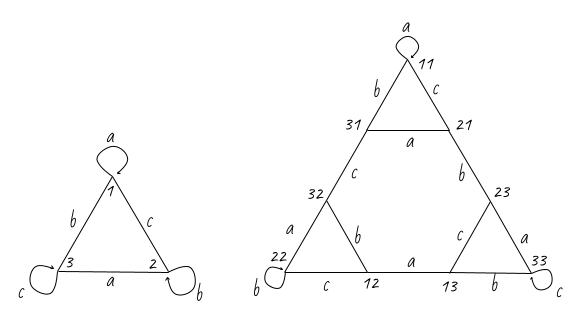
\includegraphics[scale=0.36]{H3_12.png}
	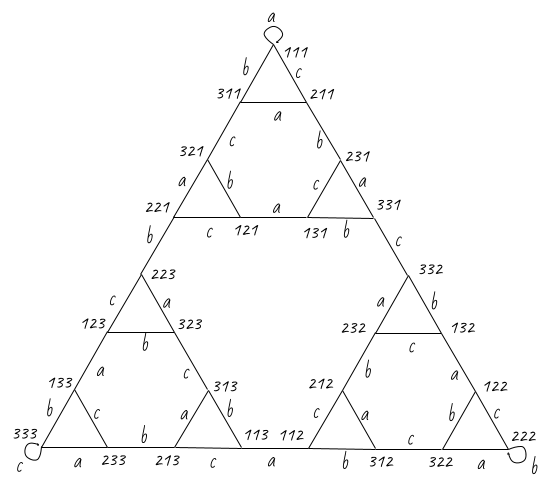
\includegraphics[scale=0.36]{H3_3.png}
	\caption{First three Schreier graphs for $H_3$}
\end{figure}

\newpage

Nevertheless, for $k \ge 4$ the sequence $H_k^n$ appears to be very complex. In \cite{Hanoi1} reader can found an asymptotic estimation of the $H_k^n$ diameter. The explicit form of the shortest path or the spectrum is an open problem even for $k = 4$. 


\begin{figure}[h]
	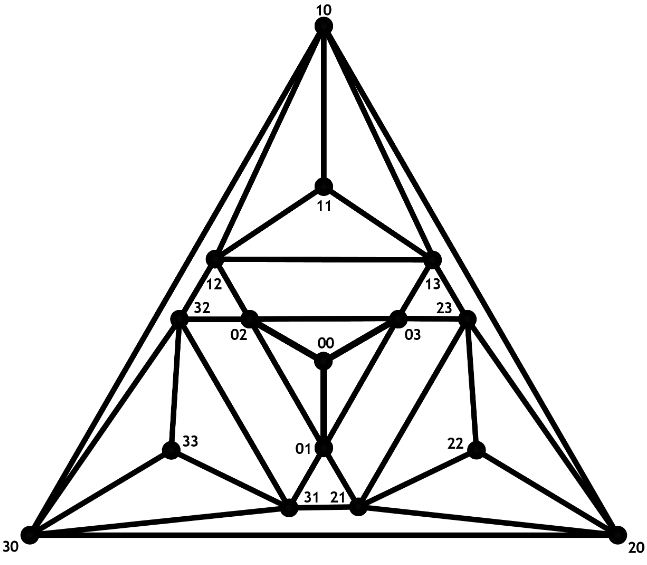
\includegraphics[scale=0.34]{H4_2.png}
	\caption{$H_4^2$ in the planar form (here disks enumerated with $\{0, 1, 2, 3\}$)}
\end{figure}

\begin{figure}[h]
	\includegraphics[scale=0.3]{H4_schreier.jpg}
	\caption{$H_4^3$ without loops}
\end{figure}

\newpage
\section{Word Problem}

\subsection{Description, algorithm, correctness}

There are three classical decision problems for finitely-generated groups: 

\begin{itemize}
	\item \textbf{The Word problem} - \textit{determine, given an arbitrary word over group generators, whether or not it represents the identity element of the group}
	
	\item \textbf{The Conjugacy problem} - \textit{determine, given two words $w_1$ and $w_2$ over group generators, whether or not they represent conjugate elements in the group}
	
	\item \textbf{The Isomorphism Problem} - \textit{determine, given two presentation, whether or not groups they represent are isomorphic.}
\end{itemize}


In this work only the first one is considered. In \cite{Bond} it was shown that there is an algorithm solving the word problem for $H_k, k \ge 3$ in subexponential time $exp(O(\log^{m-2}n))$. The algorithm depends on fact that each $H_k$ is contracting and therefore for every $w \in H_k$ it's enough just to check whether all the permutations in its tree-like structure are identical.

Although it's obvious that $a_{(ij)}a_{(ij)} = e$, the general portrait of identical elements even in $H_3$ is implicit and very difficult to construct. Nevertheless, despite the fact that it is not applicable for solving the word problem, it should be mentioned that in \cite{HRepr} a full representation of $H_3$ is obtained: 

$$ H^{(3)} = \left\langle
a, b, c,\, |\, a^2, b^2, c^2, \tau^n(w_1), \tau^n(w_2), \tau^n(w_3), \tau^n(w_4) \, \forall n \ge 0
\right\rangle $$

where $\tau$ is an endomorphism of $H_3$ defined by the substitution

$$ a \mapsto a, \quad b \mapsto b^c, \quad c \mapsto c^b$$

and where
$$ w_1 = [b, a][b, c][c, a][a, c]^b[a, b]^c[c, b] $$
$$ w_2 = [b, c]^a[c, b][b, a][c, a][a, b][a, c]^b $$
$$ w_3 = [c, b][a, b][b, c]^a[c, b]^2[b, a][b, c]^a[b, c]^a $$
$$ w_4 = [b, c]^a[a, b]^c[b, a]^2[a, c][a, b]^c[c, a][c, b] $$


\begin{figure}[h]

	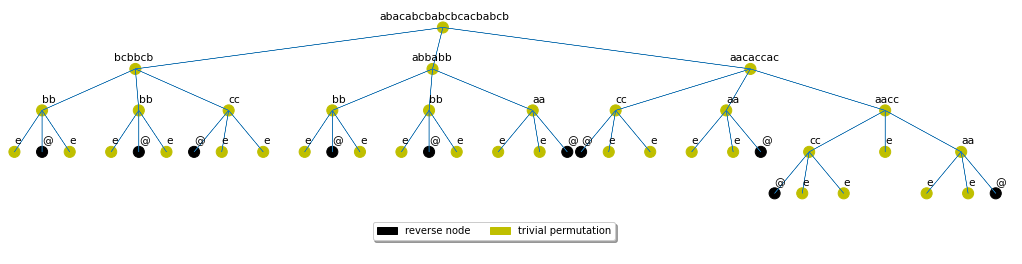
\includegraphics[scale=0.5]{non-reducible_trivial.png}
	\caption{Example of non-trivial identity element in $H_3$}
\end{figure}


Since all elements $w_x$ from the $T_w$ are being checked for their permutation, it makes sense to consider functional $size(T_w)$ that is sum of word lengths within the tree. In other words: 

\begin{equation}
\label{size}
size(w = \pi (w_1, w_2, \dots w_k)) =
\begin{cases}
0, \quad  w \in \{e, \delta\} \\
|w| + \mathlarger{\sum}_{i=1}^{k}size(w_i), \quad \text{otherwise}
\end{cases}
\end{equation}

where $\delta$ is auxiliary symbol that means recursive repetition of the word on the first level. Henceforth, for simplicity, notation $size(w)$ will be used as well as $size(T_w)$ with the same meaning. 
As an example: 

$$size(a_{(ij)}) = 1, \quad \forall (ij) \in Sym(\Sigma_k)$$
$$size(a_{(ij)}a_{(ij)} = (e, \dots, a_{(ij)}a_{(ij)}, \dots e) = 2$$


\begin{proposition}
	Complexity of the algorithm $t(w)$ solving the word problem for $w \in S_k^*$ is $O(size(T_w))$. Here $S_k$ means set of generators $a_{ij}$.
\end{proposition}

\begin{proof}
	For every vertex $w_x \in T_w$ the root permutation and its
	first-level sections can be computed in $O(|w_x|)$ operations. Thus,
	$$
	t(w) = \sum_{w_x \in T_w} O(|w_x|) = O(size(T_w)),\, \text{by definition (\ref{size})}.
	$$
	
\end{proof}
\subsection{The worst case complexity in $H_3$}


Define $X \subset H_3$ to be a set of all the elements that can be represented as periodic words over generators with 3-length word without repetitions as the period. More precisely: 

\begin{equation}
X = \left\{ (xyz)^k, \, (xyz)^k x, \, (xyz)^k xy  |\, k \in \mathbb{N}\cup\{0\}, \, x,y,z \in S_3, x \ne y \ne z \ne x   \right\}
\end{equation}

As it was already mentioned, these elements also can be interpreted as the optimal strategies in the game.

\begin{lemma}
	Any $w \in X$ will have one of the following forms:
	$$\pi (w_1, w_2, e), \quad \pi(w_1, e, w_2), \quad \pi(e, w_1, w_2), $$
	where $w_1, w_2 \in X, \quad |w_1|, |w_2| \in
	\left\{
	\left\lfloor
	\frac{n}{2}
	\right\rfloor,
	\left\lceil
	\frac{n}{2}
	\right\rceil
	\right\}, \quad |w_1| + |w_2| = n, \quad n = |w|$
	\\
\end{lemma}

\begin{proof}
	Follows from the definition of multiplication.
\end{proof}


\begin{figure}[h]
	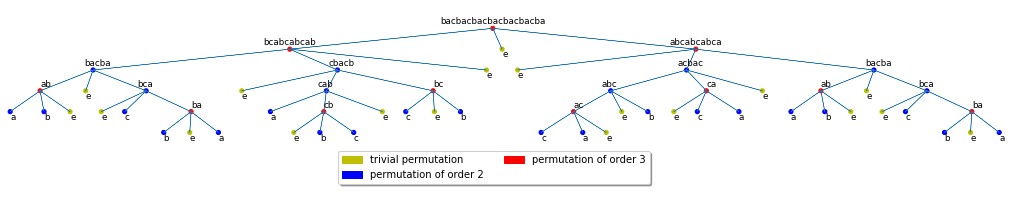
\includegraphics[scale=0.5]{../graphs/max_size_tree.png}
	\caption{Example of an element from $X$}
\end{figure}


Therefore, here is a recursive formula for calculating function $size$ (\ref{size}) for elements from $X$:

$$size(w \in X) =: a (n) = a \left(
\left\lfloor
\frac{n}{2}
\right\rfloor
\right)
+ a \left(
\left\lceil
\frac{n}{2}
\right\rceil
\right) + n, \quad a(1) = 1, \quad a(0) = 0, \quad n = |w|
$$

\begin{theorem}
	Exact form of function $a(n)$:
	\begin{equation}
	a(n) = \begin{cases}
	n \left(\left\lfloor \log_2 n + 1 \right\rfloor\right) + 2n - 2^{\left\lfloor\log_2 n\right\rfloor + 1}, \quad n > 0 \\
	a(0) = 0
	\end{cases}
	\end{equation}
\end{theorem}

\begin{proof}
	$$ a (n+1) = n + 1 + a \left(
	\left\lfloor
	\frac{n+1}{2}
	\right\rfloor
	\right)  + a \left(
	\left\lceil
	\frac{n+1}{2}
	\right\rceil
	\right) = n + 1 + a \left(
	\left\lfloor
	\frac{n}{2}
	\right\rfloor + 1
	\right) + a \left(
	\left\lceil
	\frac{n}{2}
	\right\rceil
	\right)
	$$
	
	
	$$
	\text{Let} \, b(n) := a(n + 1) - a(n) = 1 + a \left(
	\left\lfloor
	\frac{n}{2}
	\right\rfloor + 1
	\right) - a \left(
	\left\lfloor
	\frac{n}{2}
	\right\rfloor
	\right) \, \text{ - auxiliary recursion.
	}
	$$
	
	\begin{equation}
	\label{b}
	b(n) = b\left(
	\left\lfloor
	\frac{n}{2}
	\right\rfloor
	\right) + 1, \quad b(2) = 4 \quad \Rightarrow \quad b(n) = \left\lfloor \log_2{n}\right\rfloor + 3
	\end{equation}
	
	$$
	a (n + 1) = b(n) + b(n-1) + ... + b(1) =
	\sum_{1 \le k \le n} \left(
	\left\lfloor
	\log_2{k} + 3
	\right\rfloor
	\right) \quad \Rightarrow \quad a(n) = 2(n - 1) +
	\sum_{1 \le k \le n} \left(
	\left\lfloor
	\log_2{k} + 1
	\right\rfloor
	\right)  =
	$$
	$$
	= \begin{bmatrix}
	\text{amount of bits in all the} \\
	\text{numbers from} \,1 \,\text{to} \,N-1
	\end{bmatrix} = 2(n-1) + \sum_{i=1}^{\left\lfloor\log_2 n\right\rfloor} (n - 2^i) = n \left(
	\left\lfloor
	\log_2 n + 1
	\right\rfloor
	\right) + 2n - 2^{\left\lfloor\log_2 n\right\rfloor + 1}
	$$
\end{proof}


\begin{theorem}
	Elements from X have maximum $size$ among elements of length $n$, i.e.
	$$a (n) = \max (size(w) \,|\, w \in S_3^n)$$
\end{theorem}

\begin{proof}
	Induction on $n$.
	\begin{enumerate}
		\item Base: check examples of size calculation.
		\item Induction step:\\
		Let $\forall k < n \quad a (k) = \max (size(w) \,|\, w \in S_3^k)$. Consider any $w \in S_3^{n}, \, w = \pi (w_1, w_2, w_3)$. Now it shall be shown that $size(w) \le a(n)$\\
		\\
		Let $ x_1 := |w_1|, \, x_2 := |w_2|, \, x_3 := |w_3|$. If $w$ has maximum size then, due to induction hypothesis \\
		\begin{equation}
		\label{functional}
		size(w) \le a(x_1) + a(x_2) + a(x_3) + n
		\end{equation}
		(we don't know what triplet $(w_1, w_2, w_3)$ could appear in $w$, so the $\le$ symbol is used here). 
		
		Since $b(x) = a(x + 1) - a(x)$ is a monotonically increasing function (\ref{b}) value of functional (\ref{functional})
		grows as long as the difference between $w_i$. Thus,
		we are allowed to assume that $\exists i, \, w_i = e$, because otherwise
		$$size(w) \le a(x_1) + a(x_2) + a(x_3) + n \le a\left(
		\left\lfloor
		\frac{n}{2}
		\right\rfloor
		\right) + a \left(
		\left\lceil
		\frac{n}{2}
		\right\rceil
		\right) + n$$
		It's easy to check that there are only 2 possible forms of $w$ with one or more identical element at the first level: $w \in X$ or such $w = z_1 z_2 z_3 ... z_n$ that has at least one $i$ with $z_i = z_{i+1}, \, \Rightarrow \, w$ could be reduced $\Rightarrow$ $size(w) < a(n)$ due to definition.
	\end{enumerate}
	
\end{proof}


\subsection{Average case complexity in $H_3$}

Due to aforementioned theorems it's guaranteed that the word problem is solvable in $O(n\log(n))$ time, where $n$ is the word's length. However, in the real life algorithm works faster. Therefore, there is some sense to consider an average complexity instead of the worst one. 

Nevertheless, this problem is much more difficult than the worst case and the exact distribution of $size$ over all the $n$-length words is still an open problem. However, randomized experiments shows that distribution approximates $Binom(f(n), p)$ (figures \ref{figure:comparing}, \ref{figure:dist-big})

%\begin{figure}[h]
%	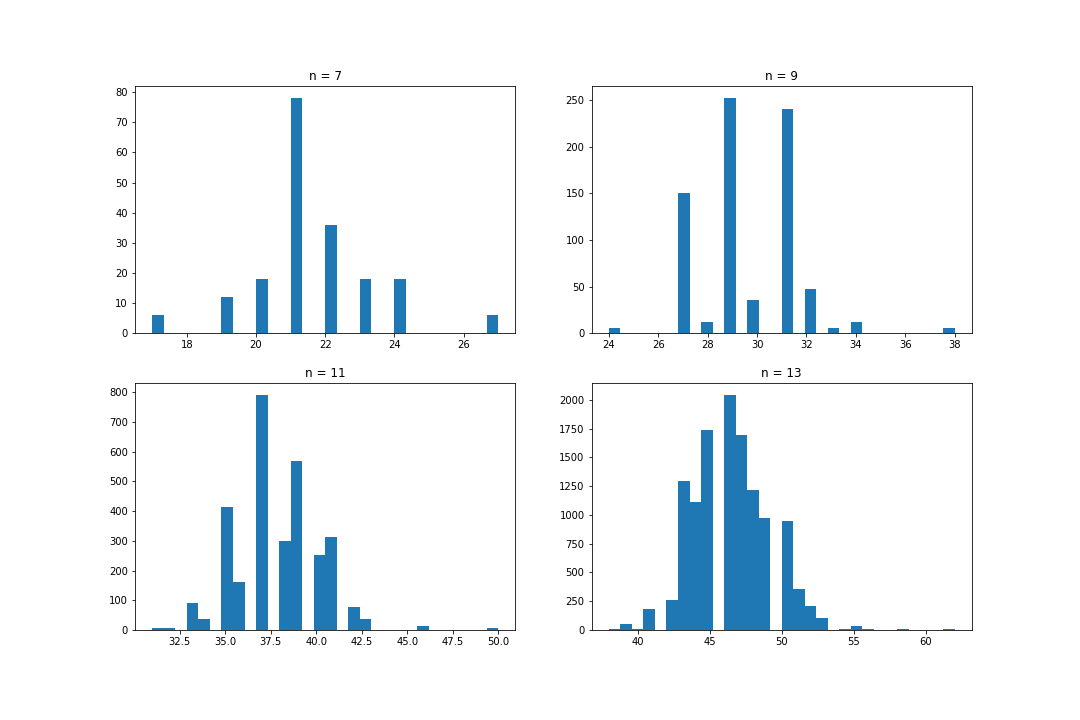
\includegraphics[scale=0.5]{size_distribution.png}
%	\caption{Full distribution of $size$ for some small $n$}
%	\label{figure:dist-small}
%\end{figure}


\begin{figure}[h]
	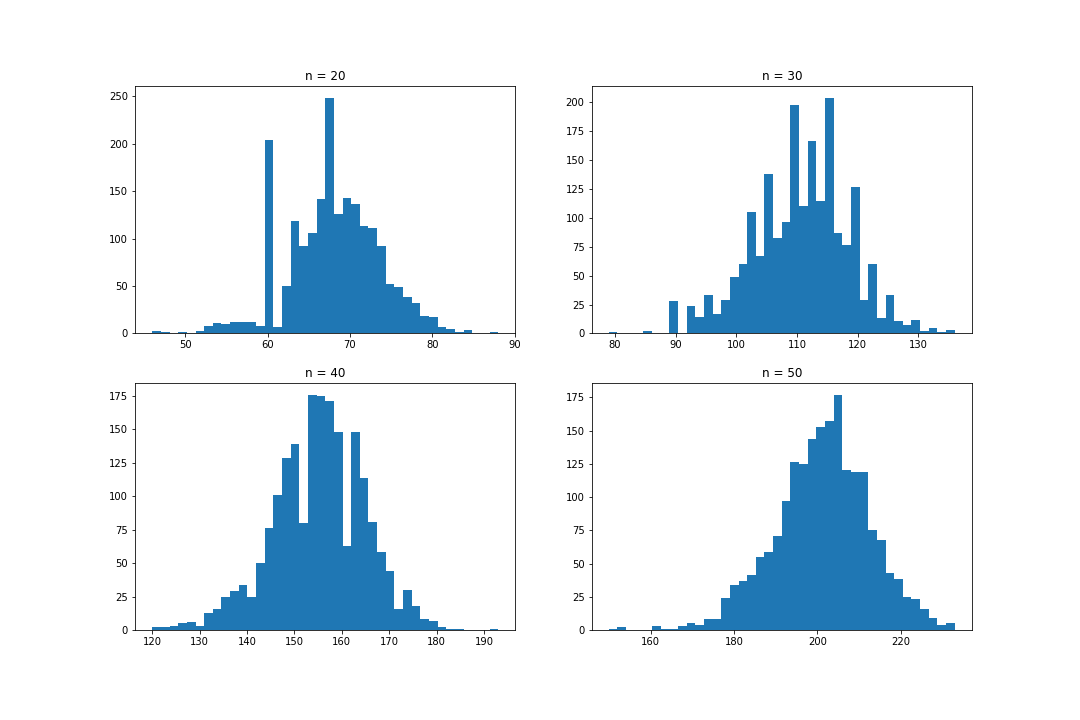
\includegraphics[scale=0.4]{size_distribution2.png}
	\caption{Distribution of $size$ of 2000 random words for some big $n$}
	\label{figure:dist-big}
\end{figure}


\begin{figure}[h]
	\raggedleft
	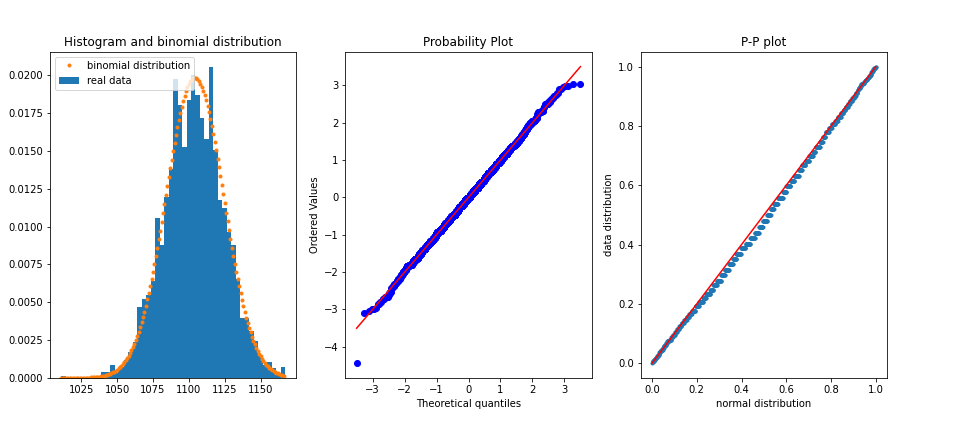
\includegraphics[scale=0.5]{size_with_binomial.png}
	\caption{Comparing $size$ of 3000 random words with $Binom(a(n), 0.633)$ and with standard normal distributions for $n = 200$}
	\label{figure:comparing}
\end{figure}


\begin{hypothesis}
	Let $\xi_n$ be the random word of length $n$ over generators and $\theta_n \sim Binom(a(n), p), \, p = const \approx 2/3$ Then 
	
	$$||size(\xi_n) - \theta_n||_2 \rightarrow 0, \, n \rightarrow \infty$$
\end{hypothesis}

If this hypothesis is true then average size of $n$-length word $\approx E(Binom(a(n), p)) = p a(n) = O(n \log n)$. 

\section{Order Problem}

Another goal of this work is to explore elements of $H_k$ of finite order. 

\subsection{Description, algorithm, correctness}

The order problem is formulated as follows: \textit{determine, given an arbitrary word over group generators, whether or not it represents an element of finite order in the group}

To construct an algorithm solving this problem consider any element $w \in H_k, \, w = \pi (w_1, w_2, \dots w_k)$.

\begin{proposition}
	\begin{equation}
		\label{order}
		order(w) = order(\pi) * lcm(order(s_i), 1 \le i \le k),
	\end{equation}
	
	where $w^{order(\pi)} = (s_1, s_2, \dots s_k)$ and $lcm$ means the least common multiplier. Note that $order(s_i)$ can be infinite. 
\end{proposition}

\begin{proof}
	Due to the multiplication rule
	
	$$(w^{order(\pi)})^n = (s_1^n, s_2^n, \dots s_k^n)$$
	
	Assuming that $order(s_i) < \infty$ for all $i$ it's enough to take $lcm(s_i, 1 \le i \le k)$ as $n$ and get the entire first level from identities. Otherwise, none of $n$ will reduce the element of infinite order. 
\end{proof}

\begin{corollary}
	\label{corollary:solvable}
	The order problem is solvable in $H_3$.
\end{corollary}

\begin{proof}
	Construct an algorithm that checks whether order of $w$ is finite. It just computes function \ref{order} recursively. 
	
	More precisely, given $w = \pi (w_1, w_2, \dots w_k)$: 
	\begin{enumerate}
		\item set $N := 1$
		\item \label{item:get-w} get $w$, set $N_w := N$
		\item calculate $w^{order(\pi)} = (s_1, s_2, \dots s_k)$, update $N = N * order(\pi)$
		\item \label{item:every-word} for every word $s_i$:
		
		\begin{itemize}
			\item if $s_i$ is $e$, skip it. If though $s_i$ is one of the atoms, return that the order is $\infty$
			\item check whether $s_i$ has already appeared at the some level before. 
			
			If so then calculate the value $N/N_{s_i}$. Hereupon it will be called \textit{length of cycle}. If it is 1 then we call it as \textit{cycle of unitary length} and just skip it. Otherwise we call it as \textit{cycle of positive length} and return that the order is $\infty$
			
			\item check whether $s_i$ is finite, passing it to the step (\ref{item:get-w}) as the new $w$. If so, continue, else return that the order is $\infty$
		\end{itemize}
		\item return that the order is finite
	\end{enumerate}
	
	Cycle of positive length means that the order will increase forever and thus, it is $\infty$. At the other hand, cycle of unitary length just means recursive repetition of itself at some level without raising to some power. It means that the root permutation is identical too. Now it shall be shown that the considered algorithm always stops in $H_3$. Due to the multiplication rule 

	\begin{equation}
		\label{equation:orbits}
		s_i = \prod_{j=1}^{order(\pi)} w_{x_j}, \quad x_j \in orbit_{\pi}(i)
	\end{equation}
	
	
	and to the definition of atoms
	
	$$|s_i| \le \sum_{j=1}^{k} |w_j| = (k-2)|w|$$
	
	Therefore, the length of $s_i$ can't increase and algorithm will eventually encounter atoms or cycle of any length. 
		
\end{proof}

As a result, there is an algorithm solving the order problem for the $H_3$. It is still an open problem whether the proposed algorithm always stops in $H_k, k \ge 4$ processing elements in the breadth-first order , i.e. whether each element $w \in H_k$ of infinite order has a cycle of positive length. Nevertheless, it can be improved: 

\begin{itemize}
	\item due to the equation \ref{equation:orbits}, $s_i$ will contain only elements $w_j, \, j \in orbit_i(\pi)$. Moreover, two different elements $s_i, s_j, \, j \in orbit_i(\pi)$ are identical up to cyclic shifting and therefore, since every atom has order 2, they are conjugated. Finally, it means that $s_i$ and $s_j$ have the same order and thus, only one element $s_i$, $i \in orbit_i(\pi)$ should be checked
	
	\item likewise during the step \ref{item:every-word} of the algorithm it's enough to check whether any cyclic shifts of $s_i$ has already appeared at some level before. Moreover, it also can be checked solving the word problem for every word has already appeared and all cyclic shifts of $s_i$ whether any pair represent the same element of the $H_k$ (despite the complexity of this checking)
\end{itemize}

However, even with these improvements the finiteness of algorithm's work is still an open problem. 

\begin{figure}[h]
	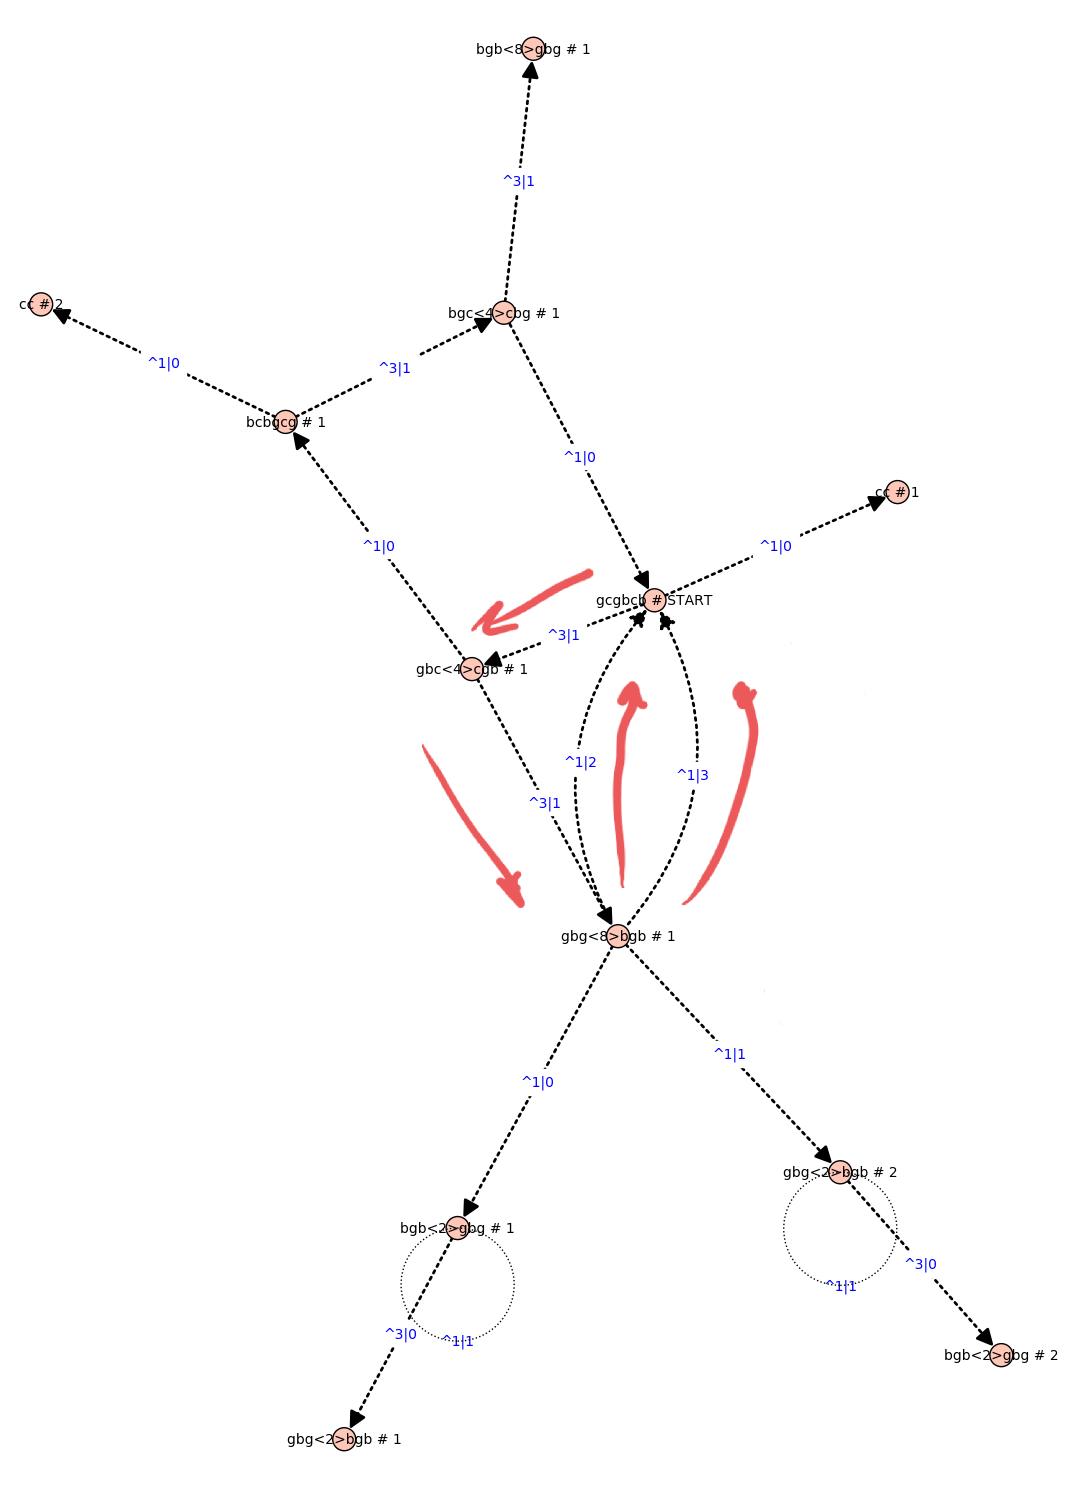
\includegraphics[scale=0.25]{order_graph.png}
	\caption{Graph that represents work of the algorithm. Vertex with label <START> means the given word $w$. Edges $\textasciicircum x | y$ mean raising to the power $x$ and making slice towards $y$}
\end{figure}



\newpage
\section{Implementation}

In this part some specifics of Python implementation of automaton groups will be described. Full code and documentation reader can find in \url{https://github.com/davendiy/automata-groups}.

\subsection{Overview}
Here is some part of documentation, that describes all the implemented classes and functions. Algorithmic specifics (structure of elements, tree drawing, multiplication) will be described after it.

\vspace{1cm}

\begin{itemize}

	\item[class] \textbf{Permutation}\textit{(form: list/tuple/int)}

	Pure Python version of \href{https://docs.sympy.org/latest/modules/combinatorics/permutations.html}{sympy.combinatorics.Permutation}. 
	
	Implements an element of the Symmetric group $S_n$. 
	
	-----------------------
	
	\vspace{0.5cm}
	\begin{itemize}
		\item[def] \textit{array\_form()}
		
		Return an array form of Permutation. 
		
		\item[def] \textit{cyclic\_form()}
		
		Return representation of the permutation as list of disjoint cycles.
		
		\item[def] \textit{order()}
		
		Return order of the Permutation.
		
		\item[attr]  \textit{size}
		
		Return size of the Permutation, i.e. $n$. 
	\end{itemize}
	
	-----------------------
	
	Examples
	
	\begin{lstlisting}[language=python]
	>>> pi = Permutation([1, 2, 0, 3])
	>>> pi.cyclic_form()
	>>> pi.cyclic_form
	[[0, 1, 2]]
	>>> pi.array_form
	[1, 2, 0, 3]
	>>> sigma = Permutation([1, 0, 3, 4, 2])
	>>> sigma.cyclic_form
	[[0, 1], [2, 3, 4]]
	>>> sigma
	Permutation([1, 0, 3, 4, 2])
	>>> str(sigma)
	'(0 1)(2 3 4)'
	>>> pi * sigma
	Permutation([0, 3, 1, 4, 2])
	>>> str(pi * sigma)
	'(1 3 4 2)'
	>>> (pi * sigma).size
	5
	>>> pi.size
	4
	>>> sigma.size
	5
	\end{lstlisting}
	
	
	\vspace{1cm}
	
	\item[class] \textbf{TriedDict}\textit{(**words)}
	
	Implementation of Dictionary based on trie a.k.a. prefix
	tree as a recursive dictionary. Note that the interface of Python dictionary is fully available and only new methods will be mentioned.
	
	-----------------------
	
	Parameters
	
	\begin{itemize}
		\item \textit{**words} : elements of the result dictionary
	\end{itemize}
	
	-----------------------
	
	\begin{itemize}
		\item[def] \textit{max\_prefix(string: str)}
		
		Get prefix of the given string with maximum length that
		contains in the TriedDict and corresponding value. 
		
		------------------
		
		Returns\\
		(\textit{found\_prefix}, \textit{left\_string}, \textit{value})
			
	\end{itemize}
	
	-----------------------
	
	Examples
	
	\begin{lstlisting}[language=python]
	>>> tr_dict = TriedDict(test=2, test2=3)
	>>> tr_dict['hello there'] = 4
	>>> print(tr_dict)
	TriedDict({'t': {'e': {'s': {'t': {'': 2, '2': {'': 3}}}}}, 'h': {'e': {'l': {'l': {'o': {' ': {'t': {'h': {'e': {'r': {'e': {'': 4}}}}}}}}}}}})
	>>> 'hello there' in tr_dict
	True
	>>> 'test3' in tr_dict
	False
	>>> del tr_dict['hello there']
	>>> 'hello there' in tr_dict
	False
	>>> tr_dict.max_prefix('test4')
	('test', '4', 2)
	>>> list(tr_dict.items())
	[('test', 2), ('test2', 3)]
	>>> list(tr_dict.keys())
	['test', 'test2']
	>>> list(tr_dict.values())
	[2, 3]
	\end{lstlisting}
	
	\vspace{1cm}
	\item[class] \textbf{Trie}\textit(*words: str)
	
	Implementation of Trie a.k.a prefix tree as a recursive dictionary. The interface of Python \textit{set} is fully available. 
	
	-----------------------
	
	Parameters
	\begin{itemize}
		\item \textit{*words} : elements for the result trie
	\end{itemize}

	-----------------------
	
	Examples

	\begin{lstlisting}[language=python]
	
	>>> trie = Trie("word", "word2", "word3", "w", "wo", "next")
	>>> print(trie)
	Trie({'w': {'o': {'r': {'d': {'': '', '2': {'': ''}, '3': {'': ''}}}, '': ''}, '': ''}, 'n': {'e': {'x': {'t': {'': ''}}}}})
	>>> 'word' in trie
	True
	>>> 'word123' in trie
	False
	>>> 'wor' in trie
	False
	>>> trie.add('word1231')
	>>> 'word1231' in trie
	True
	>>> trie.remove('w')
	>>> 'w' in trie
	False
	>>> list(trie)
	['word', 'word2', 'word3', 'word1231', 'wo', 'next']
	>>> trie.max_prefix('word123next')
	('word', '123next')
	\end{lstlisting}
	
	-----------------------

	Raises
	
	\begin{itemize}
		\item \textit{TypeError}  : when called methods \_\_getitem\_\_, \_\_setitem\_\_, \_\_delitem\_\_
	\end{itemize}

	-----------------------

	\textit{Notes}

	Trie is based on TriedDict, however it doesn't support container
	protocol and therefore doesn't have attributes keys, values and items.
	
	\vspace{1cm}
	\item[class] \textbf{Tree}\textit{(value, children)}
	
	Recursive tree structure, capable to be drawn in matplotlib.
	
	Object of this class represents a tree node with value and any amount
	of children.
	
	-----------------------
	
	Parameters
	
	\begin{itemize} 
		
		\item[-] \textit{value}: str, value that will be shown on the plot
		\item[-] \textit{children}: iterable of Tree objects
	
	\end{itemize}

	-----------------------

	\begin{itemize}
		\item[def] \textit{copy()}
		
		Create copy of the entire tree recursively.
		
		\item[def] \textit{add\_child(child, position=None)}
		
		Add copy of the child to the tree.
		
		------------------
		
		Parameters
		
		\begin{itemize}
			\item[-] \textit{child}: Tree or any another type

			If one has type of Tree, it will be copied and
			added (inserted) to the deque of children
			
			Else new Tree with the given value will be created
			
			\item[-] \textit{position}
		\end{itemize}
	
		
		\item[def] \textit{height}()
		
		Just height of tree, calculated using dfs.
		
		------------------
		
		\textit{Notes}

		Returned value isn't cached, therefore dfs will be run anyway.
		
		
		\item[def] \textit{vert\_amount}()
		
		Calculates the amount of all the vertices recursively
		using dfs.
		
		------------------
		
		\textit{Notes}
		
		Returned value isn't cached, therefore dfs will be run anyway.
		
		
		\item[def] \textit{remove(child)}
		
		Remove child from tree.
		
		------------------
		
		Parameters
		
		\begin{itemize}
			\item[-] \textit{child}: Tree or value of tree
		\end{itemize}
		
		------------------
		
		\textit{Notes}
		
		If there are more than one children with same value, only the first one will be deleted if parameter child represents value.
		
		
		\item[def] \textit{draw(start\_x=0, start\_y=0, scale=10, radius=2, fontsize=10, save\_filename='')}
		
		Draw the tree in matplotlib.
		
		------------------
		
		Parameters
		
		\begin{itemize}
			\item[-] \textit{start\_x}: x coordinate of the start position on the plane
			
			\item[-] \textit{start\_y}: y coordinate of the start position on the plane
			
			\item[-] \textit{scale}: length of one step of offset.
			Offset is measure of vertices' displacement relative to
			left upper corner. Distance between 2 generation == one
			step of offset. 
			
			\item[-] \textit{radius}: radius of vertices
			
			\item[-] \textit{fontsize}: size of font (like fontsize in matplotlib.pyplot.text)
			
			\item[-] \textit{save\_filename}: name of file, where it should be save. Default == '', means that the picture won't be saved			
		\end{itemize}

	\item[def] \textit{make\_offsets()}
	
	Calculates offsets of all the vertices relative to zero point -
	the left bound. Uses for drawing without overlaps.
	\end{itemize}
	
	
	\vspace{1cm}
	\item[class] \textbf{AutomataGroupElement}\textit(name: str, permutation: Permutation, children=None, is\_atom=False, group=None)
	
	Class that represents element of any Automaton group. 
	
	-----------------------
	
	Parameters
	
	\begin{itemize}
		\item[-] \textit{name}: symbol that represents one of generators (atoms) or word over generators
		
		\item[-] \textit{permutation}: the root permutation of element 
		
		\item[-] \textit{children}: a list of strings that represent elements of the first row of the element
		
		\item[-] \textit{is\_atom}: True if element is one of generators and its name should be in alphabet 
		
		\item[-] \textit{group}: object AutomataGroup, which represents a group wherefrom the element is given. If this parameter isn't given a lot of methods can't be executed (see docs of methods)

	\end{itemize}

	-----------------------
	
	Attributes 
	
	\begin{itemize}
		\item[-] \textit{name}: name, can't be set
		\item[-] \textit{permutation} : root permutation, can't be set
		\item[-] \textit{cardinality} : amount of children / size of the permutations, can't be set 
		\item[-] \textit{parent\_group}: group wherefrom the element. Can be set, i.e. every element can be moved from one group to another
	\end{itemize}
	
	
	-----------------------
	
	\begin{itemize}
		\item[def] \textit{dfs}()
		
		Go through the entire tree portrait of element and return all the elements on vertices in deep-first order.
		
		------------------
		
		\textit{Notes}
		
		Can't be executed if \textit{parent\_group} isn't defined.
		
		\item[def] \textit{bfs}()
		
		Go through the entire tree portrait of element and return all the elements on vertices in deep-first order

		------------------
		
		\textit{Notes}
		
		Can't be executed if \textit{parent\_group} isn't defined.
		
		\item[def] \textit{\_\_getitem\_\_(item)}
		
		Assuming \textit{item} be the word $x$ over $\{0, \dots n\}$, where $n$ is cardinality, return the slice towards this word $w|_x$
		
		------------------
		
		\textit{Notes}
		
		Can't be executed if \textit{parent\_group} isn't defined.
		
		\item[def] \textit{\_\_call\_\_(word)}
		
		Apply the group action of the element on the given word. 
		
		------------------
		
		\textit{Notes}
		
		Can't be executed if \textit{parent\_group} isn't defined.
		
		
		\item[def] \textit{\_\_mul\_\_(other)}
		
		Multiply this element by other, applying Lempel-Ziv algorithm
		
		------------------
		
		\textit{Notes}
		
		Can't be executed if \textit{parent\_group} isn't defined.
		
		
		\item[def] \textit{\_\_pow\_\_(power)}
		
		Binary raising to the power. 
		
		------------------
		
		\textit{Notes}
		
		Can't be executed if \textit{parent\_group} isn't defined.
		
		
		\item[def] \textit{inverse()}
		
		Get the inverse element of this one, i.e. raising to the (-1) power. 
		
		------------------
		
		\textit{Notes}
		
		Can't be executed if \textit{parent\_group} isn't defined.
		
		\item[def] \textit{is\_one()}
		
		Check whether the given element represents an identity of the group, solving the word problem with the proposed algorithm.
		
		------------------
		
		\textit{Notes}
		
		Can't be executed if \textit{parent\_group} isn't defined.
		
		\item[def] \textit{order(check\_finite=True)}
		
		Return the order of the element solving the order problem with proposed algorithm. If the element has infinite order, return float('inf'). Check finiteness of element if the \textit{check\_finite} is True. 
		
		------------------
		
		\textit{Notes}
		
		Can't be executed if \textit{parent\_group} isn't defined.
		
		\item[def] \textit{is\_finite()}
		
		Check whether the given element has finite order solving the order problem with proposed algorithm. 
		
		------------------
		
		\textit{Notes}
		
		Can't be executed if \textit{parent\_group} isn't defined.
		
		\item[def] \textit{order\_graph(graph)}
		
		Solve the order problem with proposed algorithm and build a directed graph of states while doing it. \textit{graph} can be any type that implements digraph interface (e.g. sage.graphs, networkx, etc). 
		
		------------------
		
		\textit{Notes}
		
		Can't be executed if \textit{parent\_group} isn't defined.
	
		\item[def] \textit{show(self, start\_x=0, start\_y=0, scale=10, radius=4, fontsize=50,
			save\_filename='', show\_full=False, y\_scale\_mul=3, lbn=False,	show\_names=True)}
		
		Draws the tree-like structure of element in matplotlib.
		
		------------------
		
		Parameters
		
		\begin{itemize}
			\item[-] \textit{start\_x}: x coordinate of the start position on the plane
			
			\item[-] \textit{start\_y}: y coordinate of the start position on the plane
			
			\item[-] \textit{scale}: length of one step of offset.
			Offset is measure of vertices' displacement relative to
			left upper corner. Distance between 2 generation == one
			step of offset. 
			
			\item[-] \textit{radius}: radius of vertices
			
			\item[-] \textit{fontsize}: size of font (like fontsize in matplotlib.pyplot.text)
			
			\item[-] \textit{save\_filename}: name of file, where it should be save. Default == '', means that the picture won't be saved		
			
			\item[-] \textit{show\_full}: False if you want elements with attribute 'simplify' to draw as just one node with name.
			
			\item[-] \textit{y\_scale\_mul}: multiplier of y-axes scale
			It's used for bigger step between generations
			
			\item[-] \textit{lbn}: leaves belong names, True if you want to print names of leaves belong them
			
			\item[-] \textit{show\_names}: True if you want to plot the names of vertices
			
		\end{itemize}
	\end{itemize}

	---------------------

	Examples
	
	\begin{lstlisting}[language=python]
	>>> H3 = AutomataGroup.generate_H3()
	>>> H3.gens
	[H3(a = (2)(0 1) (e, e, a)), H3(b = (0 2) (e, b, e)), H3(c = (1 2) (c, e, e))]
	>>> el = H3('abcabcabc')
	>>> el
	H3(abcabcabc = (0 2) (acbac, e, bacb))
	>>> el.tree.size()
	38
	>>> el.order()
	inf
	>>> el.describe()
    =====H3(abcabcabc = (0 2) (acbac, e, bacb))=====
	Group:     
	AutomataGroup H3
	over alphabet {'0', '1', '2'}
	generated by <H3(a = (2)(0 1) (e, e, a)), H3(b = (0 2) (e, b, e)), H3(c = (1 2) (c, e, e))>.
	
	size:      38
	height:    7
	
	Generation: 0, element: abcabcabc
	Generation: 1, element: bacbacbac
	Generation: 1, element: e
	Generation: 2, element: abcabcabc
	Found cycle between abcabcabc and abcabcabc of length 4.0
	
	is finite: False
	order:     inf
	
	Found cycle
	start deep:   0
	end deep:     2
	start el:     abcabcabc
	end el:       abcabcabc
	start power:  1
	end power:    4
	cycle weight: 4.0
	full path:    00
	word with cycle orbit:  (00)
	========================================
	
	>>> el.inverse()
	H3(cbacbacba = (0 2) (bcab, e, cabca))
	>>> el ** 3
	H3(abcabcabcabcabcabcabcabcabc = (0 2) (acbacbacbacbac, e, bacbacbacbacb))
	
	\end{lstlisting}
	
	
	\item[class] \textbf{AutomataGroup}\textit{(name, gens: AutomataGropElement-s, reduce\_func=id\_func, lempel\_ziv=True)}
	
	Class that represents finite-generated automaton group. 
	
	---------------------
	
	Parameters 
	
	\begin{itemize}
		\item[-] \textit{name}: name of the group. Note that only one group can have particular name
		
		\item[-] \textit{gens}: iterable of AutomataGroupElement-s, generators of the group
		
		\item[-] \textit{reduce\_func}: function that takes word over generators and reduces it removing subwords that represent identical elements. In $H_k$ it just removes repetitions, i.e. abaaba -> e.
		
		\item[-] \textit{lempel-ziv}: True if effective multiplication should be used
	\end{itemize}
	
	---------------------
	
	Examples 
	
	\begin{lstlisting}[language=python]
	>>> H3 = AutomataGroup.generate_H3()
	>>> H3.gens
	[H3(a = (2)(0 1) (e, e, a)), H3(b = (0 2) (e, b, e)), H3(c = (1 2) (c, e, e))]
	>>> H3('abca')
	H3(abca = (0 1 2) (e, ac, ba))
	>>> H3.random_el(20)
	H3(acbcabcbcacbcacacbac = (2) (cbccabc, cbabaca, abaccc))
	>>> H3.expected_words
	{'0', '1', '2'}
	>>> H3.alphabet
	['a', 'b', 'c']
	>>> 
	\end{lstlisting}
	
\end{itemize}






\subsection{Structure of elements}

It's a convenient way to represent elements of $H_k$ as $k$-ary rooted trees. However, it isn't the best way of representation due to several reasons: 

\begin{itemize}
	\item for the most situations there is no need to have a full tree but getting the first level and the root permutation is crucial
	
	\item majority of automaton groups isn't contracting and therefore the corresponding tree will be infinite
	
	\item keeping the full tree while doing some calculations (especially if we talk about the order problem) requires a huge amount of memory.
\end{itemize}

Hence, it's quite natural to handle elements of an automaton group just as $w = \pi (w_1, w_2, \dots w_n)$ and calculate the entire tree \textit{only in time of need}. 

In fact, tree-like representation is not exactly a tree because it often has cycles. Particularly in $H_k$ even atoms require some technical solution to avoid the infinite nature of tree-like structure, caused by recursive repetition of itself. For instance in $H_3$: 

$$ a := a_{(12)} = (1 2) (e, e, a_{(12)}) $$
$$ b := a_{(13)} = (1 3) (e, a_{(13)}, e) $$
$$ c := a_{(23)} = (2 3) (a_{(23)}, e, e) $$


To handle this situation an auxiliary symbol $\delta$ is used (in the source code it is @ at this time), which means the recursive repetition of itself.

\begin{figure}[h]
	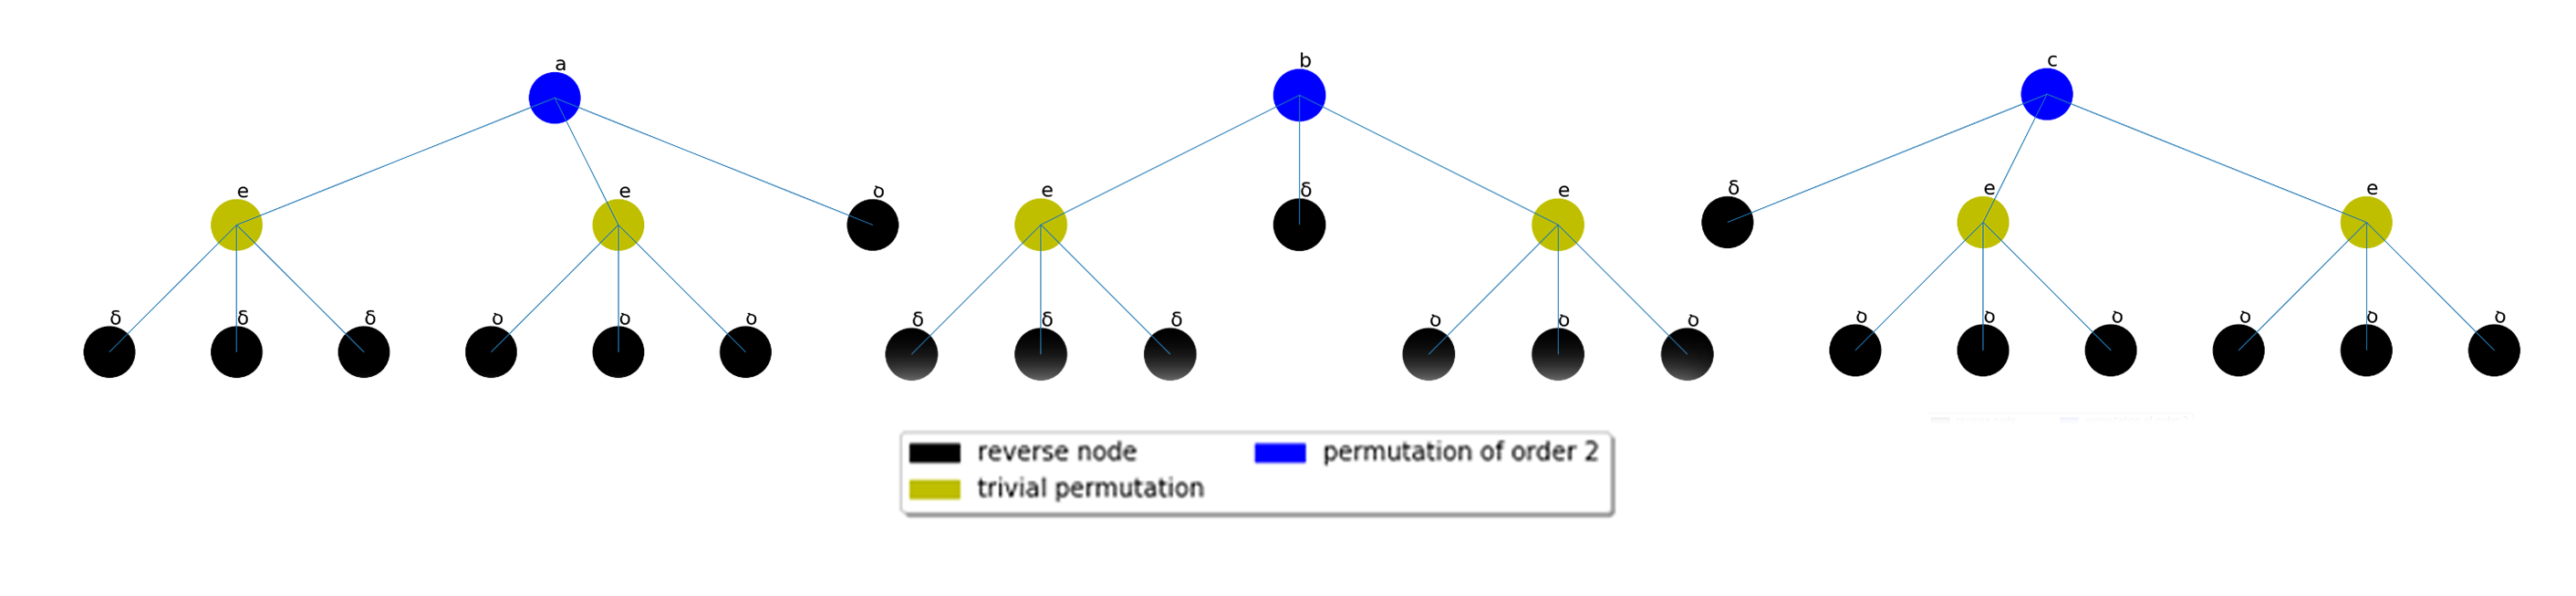
\includegraphics[scale=0.13]{a_b_c.png}
	\caption{Atoms of $H_3$}
\end{figure}


Although, it should be noted, that this technical solution isn't the best and will be replaced soon, because it doesn't handle an issue with cycles of length $>1$. As an example, consider famous Grigorchuk group generated by: 


$$a = (12)(e, e), \quad b = (a, c)$$
$$c = (a, d), \quad d = (e, b)$$  

Should we try to represent it with just $\delta$ we will get something like at Figure \ref{grigorchuk}. You can observe that at the 4-th level element $c$ was removed in order to stop the infinite recursion. 

\begin{figure}[h]	
	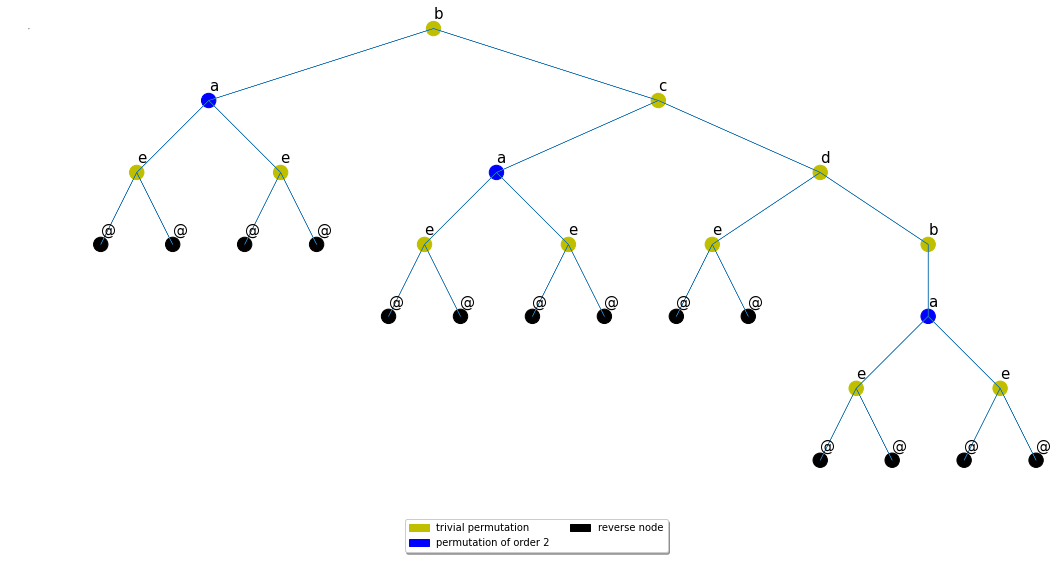
\includegraphics[scale=0.4]{grigorchuk.png}
	\caption{Tree-like structure of $b$ atom of the Grigorchuk group}
	\label{grigorchuk}
\end{figure}


\subsection{Tree drawing}

It would be great to be able to draw a tree-like structure automatically for clarity. Since all the available open-source instruments (e.g. \cite{NetworkX}, \cite{Sage-graphs}) don't provide labeling that differs from vertices' names,  own Python version was implemented just for this purpose, results of which used in this work. 


Simply, an algorithm works as follows: 

\begin{lstlisting}
Given tree T. 
    1. draw each child of T recursively 
    2. shift each child to the right position 
    3. draw the root above just in the middle 
\end{lstlisting}

The main problem is the 2-nd step because it's not completely clear what does \textit{right position} mean. For this purpose such property about vertices is used. 

\begin{definition}
	\textbf{Offset} of vertex $\phi : V \rightarrow \mathbb{R}+$ is defined recursively:
	
	\begin{itemize}
		\item $\phi(v) = 0$ for a tree with only 1 vertex
		
		\item given $T = w (T_1, T_2, \dots T_n)$, where $w$ is the root and $T_i$ are children. Consider $\phi_i$ as offset functions for each $T_i$ separately and $x_i = max({\phi_i(v), v \in T_i})$. Then for $v \in T_i$ 
		
		$$\phi(v) = \sum_{j = 1}^{i} (x_j + 1) + \phi_i(v)$$
		
		and for the root: 
		
		$$\phi(w) = \frac{1}{n} \sum_{i=1}^{n} (x_i + 1)$$
	\end{itemize}
\end{definition}


\begin{proposition}
	If a tree is drawn using offset $\phi$ and deep as coordinates of each vertex $(x, y)$ respectfully, there will be no intersections of edges.
\end{proposition}

Applying different scales for $(x, y)$ coordinates and using different radius of circles that represent vertices, we will get a result similar to the figures in this work.

\subsection{Effective multiplication}

Solving the order problem it often happens to handle huge words (up to $10^6$ letters). Standard way to find out the permutation and the first level of a word is just to multiply all the letters-atoms. Therefore, complexity of the naive algorithm is $O(n)$, which could be very time consuming if you have to do hundreds of them. Besides, since the alphabet is small for the most cases, there are multitudes of repetitive patterns within the huge word (just like in DNA). Thus, an inspiration appears to use somehow Lempel-Ziv-like (\cite{Lempel-Ziv}) algorithm herein.   

Assuming every result of multiplication is being cached the algorithm can be described in the following way: 

\begin{lstlisting}
Input data: a huge word w
            a dictionary of already processed elements (with restriction on the maximum length)
Output: permutation and the first level of w

    1. set res := e - identical element
    2. set v := the longest prefix of w that is stored in the dictionary
    3. res := res * v  - multiplication with caching 
    4. while w isn't empty go to (1)
    5. return res
\end{lstlisting}

Complexity of this algorithm is connected to the famous Lempel-Ziv complexity of finite words (check \cite{Lempel-Ziv2}) and it is out of scope of this work. 

Algorithm will be even more effective, if the dictionary is implemented as trie data structure. \cite{Algorithms} 


\newpage

\begin{thebibliography}{9}
	\bibitem{Hanoi1}
	\href{https://arxiv.org/abs/math/0601592}{Rostislav Grigorchuk, Zoran Sunik. Asymptotic aspects of Schreier graphs and Hanoi Towers groups. Department of Mathematics, Texas A\&M University, MS-3368, College Station, TX, 77843-3368, USA, 2006}
	
	\bibitem{Hanoi2}
	\href{https://arxiv.org/abs/0711.0068}{Rostislav Grigorchuk, Zoran Sunik. SCHREIER SPECTRUM OF THE HANOI TOWERS GROUP ON THREE PEGS 2007}
	
	\bibitem{Auto}
	R.I. Grigorchuk, V.V. Nekrashevich, V.I. Sushchanskiı, Automata, dynamical systems, and groups, Tr. Mat. Inst. Steklova 231 (2000) 134-214
	(Din. Sist., Avtom. i Beskon. Gruppy).
	
	\bibitem{HRepr}
	Bartholdi, Laurent; Siegenthaler, Olivier; Zalesskii, Pavel. The congruence subgroup problem for branch groups,Israel  J.  Math.187(2012),419450.
	
	\bibitem{HaoniDesk} Andreas M. Hinz,The Tower of Hanoi, Enseign. Math. (2)35(1989),
	no. 3-4, 289–321. MR MR1039949 (91k:05015)
	
	\bibitem{Bousch} \href{https://web.archive.org/web/20170921001150/https://pdfs.semanticscholar.org/fb87/0a772baf96a2e11901122a2b04c3dd25596d.pdf}{Bousch, T. (2014). "La quatrieme tour de Hanoi". Bull. Belg. Math. Soc. Simon Stevin. }
	
	\bibitem{Frame-Stewart} \href{https://core.ac.uk/download/pdf/81954097.pdf}{Klavzar, Sandi; Milutinovi, Uro; Petrb, Ciril (2002). "Variations on the Four-Post Tower of Hanoi Puzzle"}
	
	\bibitem{Hanoi Graphs Random walks}
	\href{https://scholar.rose-hulman.edu/rhumj/vol20/iss1/6}{Egler, Stephanie (2019) "Graphs, Random Walks, and the Tower of Hanoi," Rose-Hulman Undergraduate Mathematics Journal: Vol. 20 : Iss. 1 , Article 6.}
	
	\bibitem{Gray-codes}
	\href{https://web.archive.org/web/20040821062630/http://occawlonline.pearsoned.com/bookbind/pubbooks/miller2_awl/chapter4/essay1/deluxe-content.html}{Miller, Charles D. (2000). "Ch. 4: Binary Numbers and the Standard Gray Code". Mathematical Ideas (9 ed.). Addison Wesley Longman. ISBN 978-0-321-07607-6.}
	
	\bibitem{Bond}
	\href {https://arxiv.org/abs/1409.0119}{Ievgen Bondarenko "The word problem in Hanoi Towers groups" Algebra and Discrete Mathematics. Volume 17 (2014). Number 2, pp. 248 – 255}
	
	\bibitem{Sage-graphs}
	Sage reference manual >> Graph Theory \url{https://doc.sagemath.org/html/en/reference/graphs/index.html}
	
	\bibitem{NetworkX}
	NetworkX Network Analysis in Python \url{https://networkx.org/}
	
	\bibitem{Lempel-Ziv}
	\href{https://courses.cs.duke.edu/spring03/cps296.5/papers/welch_1984_technique_for.pdf}{Welch, Terry (1984). "A Technique for High-Performance Data Compression" (PDF). Computer. 17 (6): 8–19.}
	
	\bibitem{Lempel-Ziv2}
	\href{https://ieeexplore.ieee.org/document/1055501}{Abraham Lempel and Jacob Ziv, « On the Complexity of Finite Sequences », IEEE Trans. on Information Theory, January 1976, p. 75–81, vol. 22, n°1}
	
	\bibitem{Algorithms}
	\href{https://algs4.cs.princeton.edu/52trie/}{Algorithms, 4th Edition by Robert Sedgewick and Kevin Wayne, 5.2 Tries }
	
	\bibitem{Iterated-monodromy}
	\href{https://www.math.tamu.edu/~grigorch/publications/standrews.pdf}{Rostislav Grigorchuk Zoran Sunic Department of Mathematics Texas A\&M University "SELF-SIMILARITY AND BRANCHING IN GROUP THEORY", MS-3368 College STation, TX 77843-3368USA}
	
\end{thebibliography}

\newpage
\thispagestyle {empty}

\begin{appendices}
\end{appendices}
\end{document}
